\documentclass[12pt,letterpaper,boxed]{hmcpset}
\usepackage{float}
\restylefloat{figure}
\usepackage{graphicx}
\usepackage{amsmath}


\name{Lujia Zhang}
\class{CSSE 477}
\mailbox{CM 1405}
\assignment{Assignment 5}

\begin{document}

\section*{Problem 1}
IConnectionMonitor: It's an interface that runs and stops the p2p connection.\newline \newline 
IHandler: It's an interface that provides entry for IRequestHandler, IResponseHandler and AbstractHandler. \newline \newline
IHost: It's an interface that provides the information of the address and port of the host. \newline \newline
IP2PMediator: It's an interface that handles all the communication between clients and process most of the activities.\newline \newline
IPacket: It's an interface that gets the useful information from the packet such as protocol, command and object. Then it serializes and deserialize the stream. \newline \newline
IProtocol: It's an interface that controls the request and response handlers. \newline \newline
IRequestHandler: It's an interface that handles the request package. \newline \newline
IResponseHandler: It's an interface that handles the response package. \newline \newline
IStreamMonitor: It's an interface that allows to run and stop the p2p stream with multi thread enviroment. \newline \newline
AbstractHandler: It's an abstract class that creates and returns the IP2Mediator. 
\section*{Problem 2}
IActivityListener: It's an API that performs the activity. \newline \newline
IConnectionListener: It's an interface that listens to the connection, add and remove elements to the peerListModel. \newline \newline
IDownloadListener: It's an interface that provides the status of the download situation. \newline \newline
IListingListener: It's an interface that posts the status of the listing, clear the filelistmodel, then add the element to the filelistmodel. \newline \newline
IRequestLogListener: It's an interface that clears the requestLogListModel then add command and object Element to the requestLogListModel. \newline \newline
\section*{Problem 3}
\begin{figure}[H]
  \centering
  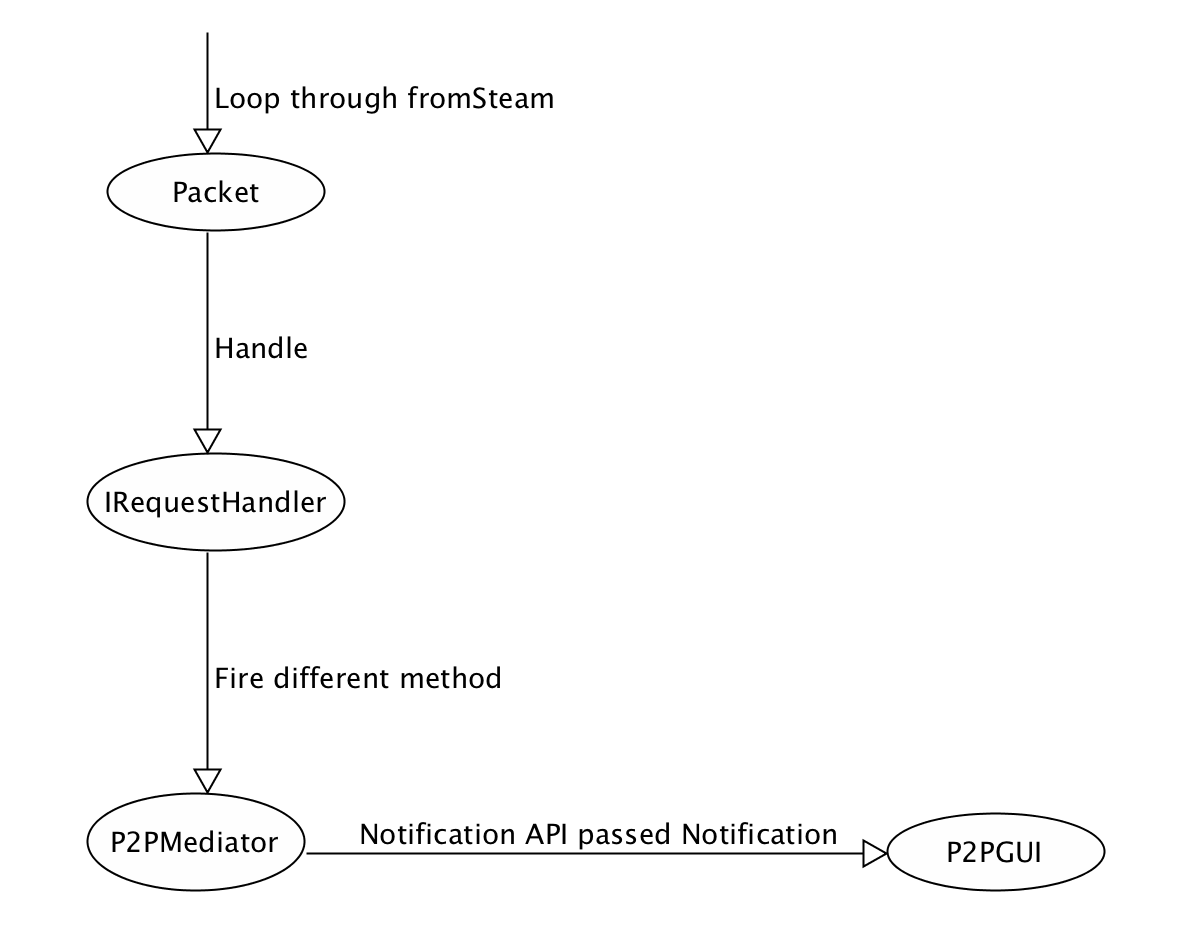
\includegraphics[width = 1.0\textwidth]{P3.png}
\end{figure}
The Packet loops through the fromStream method to parseStatus and parseHeaders, then set up protocol and handler. Then IRequestHandler handles the request. Pass to P2PMediator, it will fire different method. Then P2PGUI will get notification from the Notification API. \newline
\begin{figure}[H]
  \centering
  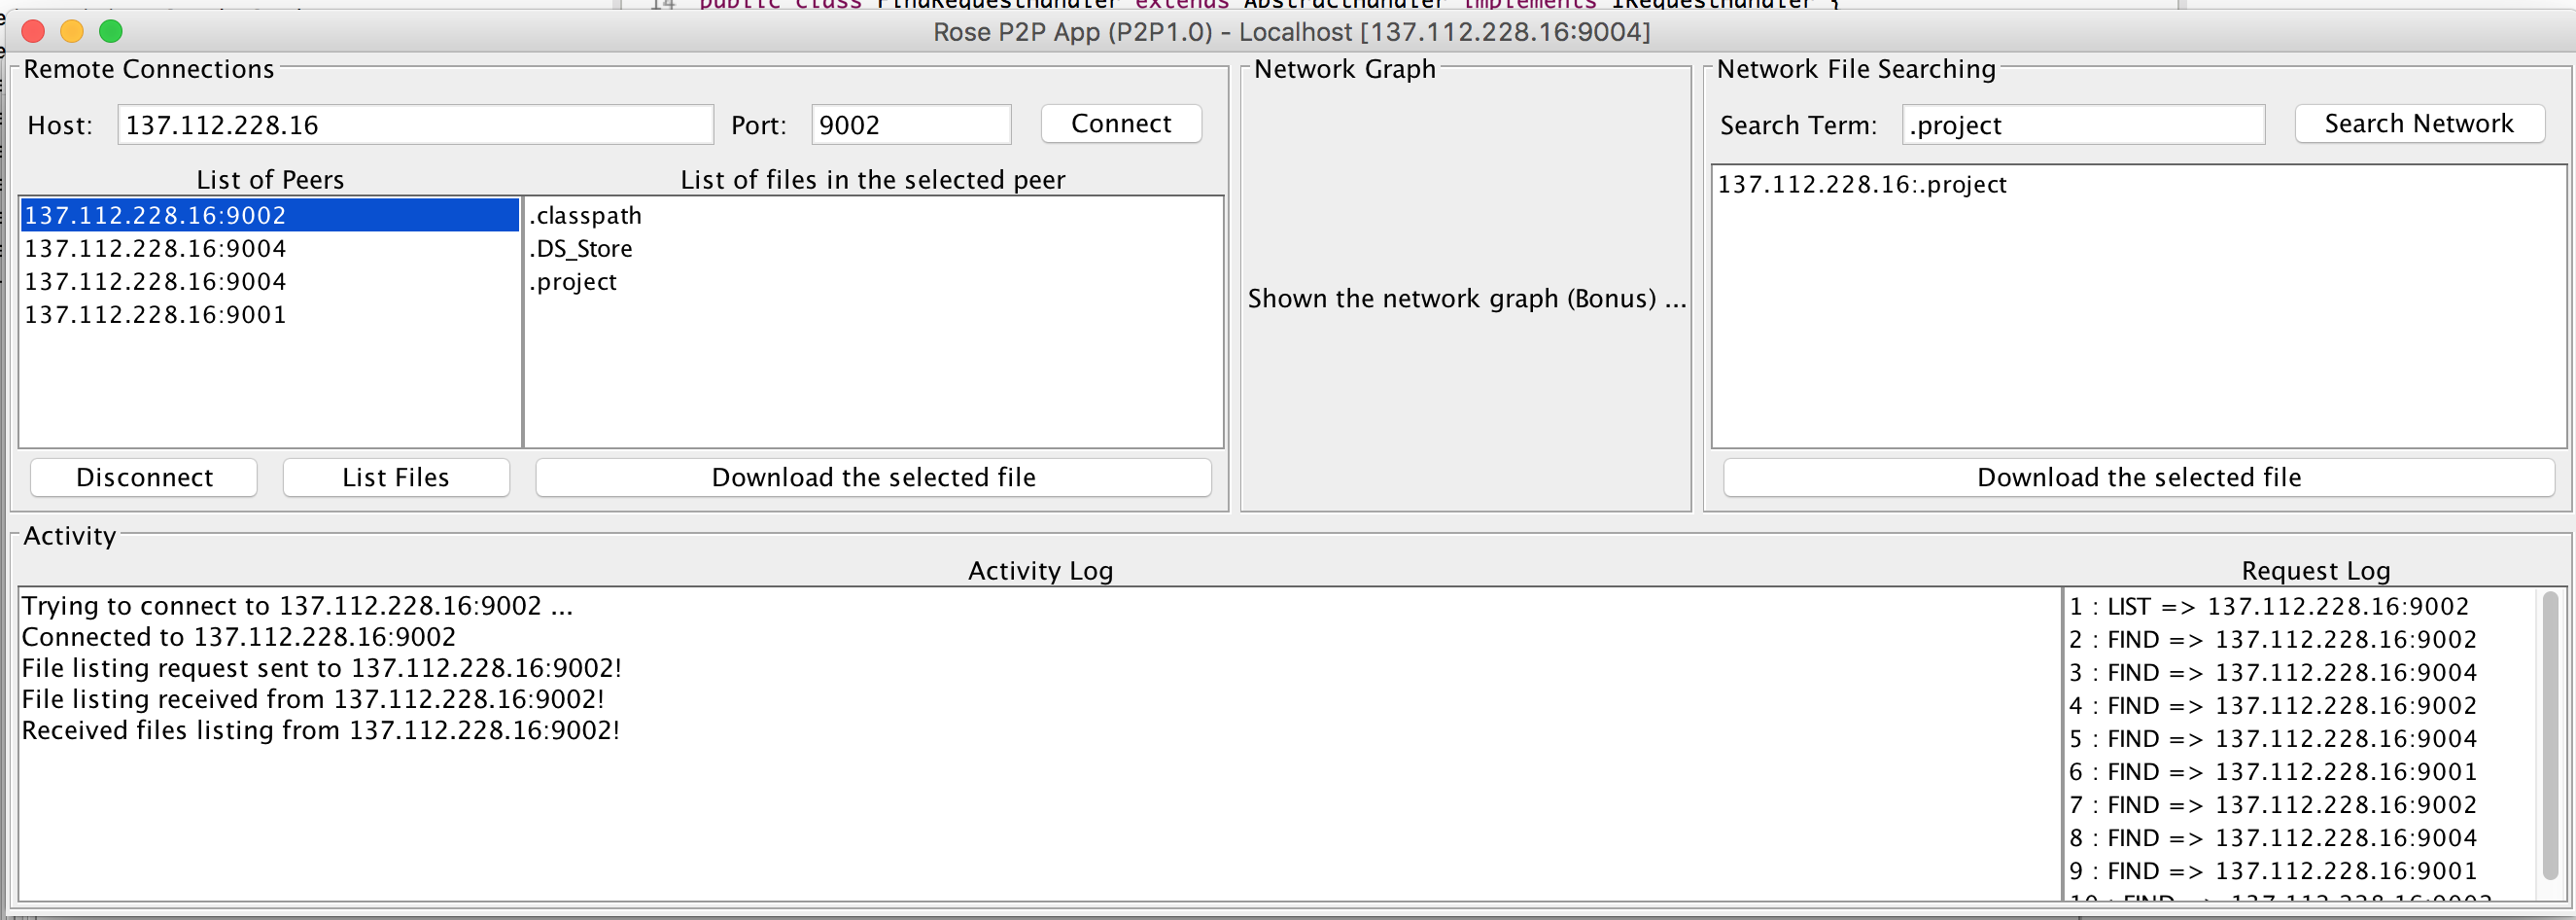
\includegraphics[width = 1.0\textwidth]{1.png}
\end{figure}
The FIND file request has format:\newline
P2P1.0 FIND $<REceiver-IP:Port><CRLF>$ \newline
$Host:<Sender-IP><CRLF>$\newline
$Port:<Sender-Port><CRLF>$\newline
$SEQ_NUM:<Sender-Generated-Seq-No><CRLF>$\newline
$ORIGINAL_HOST:<Original-Host><CRLF>$\newline
$ORIGINAL_PORT:<Original-Port><CRLF>$\newline
$DEPTH:<Search-Depth><CRLF>$\newline
$SEARCH_TERM:<Search-Term><CRLF>$\newline
$<CRLF>$\newline
The FOUND file request has format:\newline
P2P1.0 FOUND $<REceiver-IP:Port><CRLF>$ \newline
Host:$<Sender-IP><CRLF>$\newline
Port:$<Sender-Port><CRLF>$\newline
$SEQ\_NUM:<Sender-Generated-Seq-No><CRLF>$\newline
$Payload-Size:<Size-Of-Payload><CRLF>$\newline
$<CRLF>$\newline
a.txt$<CRLF>$\newline
a.gif$<CRLF>$\newline

\end{document}